\section{Vectors}

A vector is a mathematical object with magnitude and direction. In coordinates, a vector in the plane may be written as
\[
\mathbf{v}=(v_x,v_y),
\]
and a vector in space as
\[
\mathbf{v}=(v_x,v_y,v_z).
\]
The numbers \(v_x\), \(v_y\), and \(v_z\) are called components. They depend on the coordinate system.

\begin{examplebox}
The vector
\[
\mathbf{v}=(3,4)
\]
has magnitude
\[
|\mathbf{v}|=\sqrt{3^2+4^2}=5.
\]
\end{examplebox}

\begin{center}
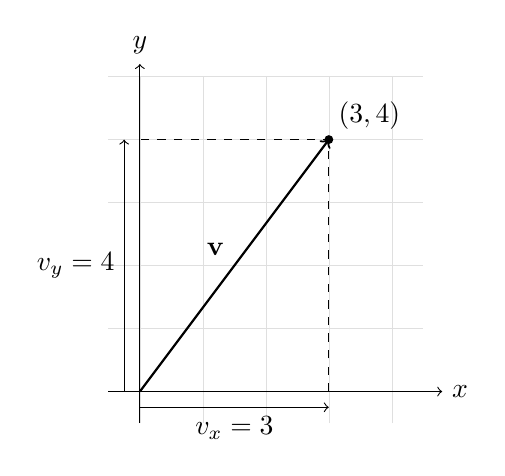
\begin{tikzpicture}[scale=0.8]
    \draw[step=1, gray!25, very thin] (-0.5,-0.5) grid (4.5,5.0);
    \draw[->] (-0.5,0) -- (4.8,0) node[right] {$x$};
    \draw[->] (0,-0.5) -- (0,5.2) node[above] {$y$};
    \draw[->, thick] (0,0) -- (3,4) node[midway, above left] {$\mathbf{v}$};
    \draw[dashed] (3,0) -- (3,4) -- (0,4);
    \draw[->] (0,-0.25) -- (3,-0.25) node[midway, below] {$v_x=3$};
    \draw[->] (-0.25,0) -- (-0.25,4) node[midway, left] {$v_y=4$};
    \fill (3,4) circle (2pt);
    \node[above right] at (3,4) {$(3,4)$};
\end{tikzpicture}
\end{center}

Vectors can be added component by component:
\[
(1,2)+(3,4)=(4,6).
\]
They can be multiplied by a scalar:
\[
2(1,3)=(2,6).
\]
The zero vector is \(\mathbf{0}=(0,0)\) in the plane and \(\mathbf{0}=(0,0,0)\) in space.

The dot product of two vectors is defined by
\[
\mathbf{a}\cdot\mathbf{b}=a_xb_x+a_yb_y
\]
in two dimensions, and by
\[
\mathbf{a}\cdot\mathbf{b}=a_xb_x+a_yb_y+a_zb_z
\]
in three dimensions.

The dot product is also related to the angle between vectors:
\[
\mathbf{a}\cdot\mathbf{b}=|\mathbf{a}|\,|\mathbf{b}|\cos\theta.
\]
This formula shows that the dot product contains information about both lengths and direction.
